\documentclass[11pt]{article}

\usepackage[margin=1in]{geometry}
\usepackage[T1]{fontenc}
\usepackage[utf8]{inputenc}
\usepackage{lmodern}
\usepackage{microtype}
\usepackage{amsmath,amssymb,amsthm,mathtools,bm}
\usepackage{array,booktabs,longtable,tabularx}
\usepackage{xcolor}
\usepackage{hyperref}
\usepackage{bookmark}
\usepackage{fancyhdr}
\usepackage{titlesec}
\usepackage{enumitem}
\usepackage{setspace}
\usepackage{needspace}
\usepackage{caption}
\usepackage{float}
\usepackage{tikz}
\usetikzlibrary{arrows.meta,positioning,calc}

\definecolor{TitleBlue}{HTML}{16324F}
\definecolor{AccentBlue}{HTML}{2A5B84}
\definecolor{SoftBlue}{HTML}{EEF4FA}
\definecolor{SoftGray}{HTML}{F5F7FA}
\definecolor{MutedText}{HTML}{4F5B66}
\definecolor{RuleGray}{HTML}{D7E1EA}
\definecolor{LineBlue}{HTML}{C9D7E4}

\hypersetup{
  colorlinks=true,
  linkcolor=AccentBlue,
  citecolor=AccentBlue,
  urlcolor=AccentBlue,
  pdftitle={Exact global insertion rule and the local-to-global theorem in Type-1, N=3 Landau-Zener},
  pdfauthor={OpenAI},
  bookmarksopen=true,
  bookmarksnumbered=true
}

\pagestyle{fancy}
\fancyhf{}
\fancyhead[L]{\textcolor{MutedText}{Type-1, $N=3$ Landau-Zener}}
\fancyhead[R]{\textcolor{MutedText}{Exact global insertion rule}}
\fancyfoot[C]{\textcolor{MutedText}{\thepage}}
\setlength{\headheight}{14pt}

\titleformat{\section}{\Large\bfseries\color{TitleBlue}}{\thesection}{0.7em}{}
\titleformat{\subsection}{\large\bfseries\color{AccentBlue}}{\thesubsection}{0.6em}{}
\titleformat{\subsubsection}{\normalsize\bfseries\color{TitleBlue}}{\thesubsubsection}{0.5em}{}

\setlength{\parindent}{0pt}
\setlength{\parskip}{0.55em}
\setlist[itemize]{leftmargin=1.4em,itemsep=0.25em,topsep=0.25em}
\setlist[enumerate]{leftmargin=1.6em,itemsep=0.25em,topsep=0.25em}
\onehalfspacing
\numberwithin{equation}{section}

\newtheorem{theorem}{Theorem}[section]
\newtheorem{proposition}[theorem]{Proposition}
\newtheorem{corollary}[theorem]{Corollary}
\newtheorem{lemma}[theorem]{Lemma}
\theoremstyle{definition}
\newtheorem{definition}[theorem]{Definition}
\newtheorem{remark}[theorem]{Remark}

\newcommand{\C}{\mathbb C}
\newcommand{\PP}{\mathbb P}
\newcommand{\ii}{\mathrm i}
\newcommand{\dd}{\mathrm d}
\newcommand{\Disc}{\operatorname{Disc}}
\newcommand{\Res}{\operatorname{Res}}
\newcommand{\red}{\operatorname{red}}
\newcommand{\im}{\operatorname{Im}}
\newcommand{\re}{\operatorname{Re}}
\newcommand{\diag}{\operatorname{diag}}
\newcommand{\id}{\mathrm{Id}}
\newcommand{\E}{\mathcal E}
\newcommand{\CY}{\Sigma_Y}
\newcommand{\CRcurve}{\Sigma_R}
\newcommand{\Chat}{\widehat{\mathcal C}}
\newcommand{\CR}{\mathfrak C_R}
\newcommand{\Hx}{\mathsf H_x}
\newcommand{\Yop}{\mathsf Y}
\newcommand{\Rop}{\mathsf R}
\newcommand{\sigmaPauli}{\sigma_3}
\newcommand{\LH}{L_H}
\newcommand{\wall}{\mathcal W}
\newcommand{\Aact}{\mathcal A_v}
\newcommand{\Ssp}{\mathcal S_v}
\newcommand{\Lin}{L_{\mathrm{in}}}
\newcommand{\Lout}{L_{\mathrm{out}}}
\newcommand{\Jact}{J^{\mathrm{act}}_{v,\theta}}
\newcommand{\Jemb}{\mathbf J_{v,\theta}}
\newcommand{\Tin}{T^{\mathrm{in}}_{\gamma}}
\newcommand{\Tout}{T^{\mathrm{out}}_{\gamma}}
\newcommand{\Tfun}{\mathcal T}
\newcommand{\Selcand}{\mathrm{Sel}^{\mathrm{cand}}_\theta(H)}
\newcommand{\Selact}{\mathrm{Sel}^{\mathrm{act}}_\theta(H)}
\newcommand{\Borel}{\mathfrak B}
\newcommand{\Jclass}{\mathfrak J_s(H)}

\newcolumntype{Y}{>{\raggedright\arraybackslash}X}
\newcolumntype{P}[1]{>{\raggedright\arraybackslash}p{#1}}
\renewcommand{\arraystretch}{1.17}

\newcommand{\infobox}[1]{%
  \begin{center}
  \fcolorbox{RuleGray}{SoftBlue}{%
    \begin{minipage}{0.93\linewidth}
    \small #1
    \end{minipage}}
  \end{center}}

\begin{document}

\begin{titlepage}
\thispagestyle{empty}
\centering
\vspace*{1.0cm}

{\Large\color{AccentBlue}\bfseries Internal theorem note\par}
\vspace{0.7cm}

{\fontsize{24}{28}\selectfont\bfseries\color{TitleBlue}Exact global insertion rule\par}
\vspace{0.15cm}
{\fontsize{19}{23}\selectfont\bfseries\color{TitleBlue}and the local-to-global theorem\par}
\vspace{0.15cm}
{\fontsize{18}{22}\selectfont\bfseries\color{TitleBlue}in Type-1, $N=3$ Landau-Zener\par}
\vspace{0.3cm}
{\Large\color{AccentBlue}\bfseries Proof record from the present conversation\par}

\vspace{0.95cm}

\begin{minipage}{0.90\textwidth}
\small
This note formalizes the last remaining generic symbolic step after the previously memorialized proofs of
\begin{enumerate}
  \item selector sufficiency in the generic simple local case, and
  \item outer-frame descent after resolved-sheet lift and half-form regularization.
\end{enumerate}
It does three things.
\begin{enumerate}
  \item It gives a precise definition of the \emph{exact global insertion rule} attached to an active selector point.
  \item It proves the \emph{exact local-to-global theorem}: a path crossing a simple active selector wall factors exactly into ordinary propagation, one embedded scalar local block on the active $2\oplus 1$ splitting, and ordinary propagation again.
  \item It records the immediate corollary that the broken morphism $j_{H,\theta}$ in the formal strategy diagram is now explicit in the generic simple regime.
\end{enumerate}

\medskip
\textbf{Scope.} Throughout, nongeneric collision scenarios are excluded: no degenerate transport ramification, no common $Q_4$-$W_4$ collision, no ordinary turning point inside the selector disk, and no spectator-gap collapse.
\end{minipage}

\vfill

{\large\color{MutedText}\today\par}
\end{titlepage}

\tableofcontents
\clearpage

\section{Executive summary}

At the April 18 baseline, the canonical gluing theorem, the exact two-sheet torus theorem, the local scalar selector multiplier, and the formal continuation-graph machinery were already in place, but the explicit local activation--multiplier morphism and the exact local-to-global insertion theorem were still open. The conversation then supplied the missing local inputs: the bridge lemma after resolved-sheet lift / half-form regularization, and the generic simple local selector sufficiency theorem. The only remaining symbolic task was therefore the exact global insertion rule.

\infobox{%
\textbf{Main theorem proved in this note.}

Let $s$ be an active selector point determined by a simple phase-active transport ramification point $v$. Then the exact continuation across $s$ is governed by a canonically embedded scalar local block:
\[
\Jemb(q;H)=\iota_v\!\bigl(I+s^{\mathrm{BS}}_{v,\theta}(q;H)N_{v,\theta}\bigr),
\]
where $q$ is any admissible overlap point in the local selector annulus, $N_{v,\theta}$ is the rank-one nilpotent determined by the crossing orientation, and $\iota_v$ acts on the active rank-two bundle and is the identity on the spectator line. For every global continuation path $\gamma$ that crosses the selector wall once and transversely,
\[
\Tfun_\gamma(H,\theta)=\Tout(q;H,\theta)\,\Jemb(q;H)\,\Tin(q;H,\theta).
\]
This factorization is exact and independent of the chosen overlap point, overlap annulus, and selector-disk radius. Equivalently, the only effect of crossing the active selector wall is the insertion of one embedded scalar local block in the active $2\oplus 1$ splitting.
}

The proof is short once the local ingredients are in hand. The bridge lemma identifies the intrinsic resolved-sheet / half-form frame with the quotient-ring / adiabatic half-form frame up to one constant geometry-only matrix, and with matched normalization that matrix is the identity. The local sufficiency theorem shows that the active two-sheet block is exactly the scalar Airy renormalization
\[
I+s^{\mathrm{BS}}_{v,\theta}(q;H)N_{v,\theta}.
\]
The spectator line is analytic across the selector wall, so the local block embeds as a direct sum with the identity. Path concatenation then gives the exact global factorization, and moving the overlap point only changes the two adjacent ordinary propagators by compensating exact sector propagators.

\section{Standing inputs and generic hypotheses}

\subsection{Type-1 geometry and continuation conventions}

We work in the Type-1, $N=3$ setting with the standard rational parametrization
\begin{equation}
\label{eq:uE}
 u(\lambda)=\frac{n(\lambda)}{p(\lambda)},
 \qquad
 E(\lambda)=\frac{m(\lambda)}{p(\lambda)},
 \qquad
 q_u(\lambda)=u\,p(\lambda)-n(\lambda),
\end{equation}
and quotient-ring fiber
\begin{equation}
\label{eq:Eu}
 \E_u=\C[\lambda]/(q_u(\lambda)).
\end{equation}
The gauged adiabatic evolution is
\begin{equation}
\label{eq:adiabatic}
 f_i'(u)=-\sum_{j\neq i}S_{ij}(u)f_j(u)+\ii\bigl(E_i(u)-E_x(u)\bigr)f_i(u),
\end{equation}
while the quotient-ring reduction is
\begin{equation}
\label{eq:reduced}
 \partial_u[R]=\ii\bigl[(m-E_xp)s_uR\bigr]=\ii\,\Hx[R],
 \qquad
 p s_u\equiv 1\pmod{q_u}.
\end{equation}
We use the common/spinor cover notation, the commuting triple $(\Hx,\Yop,\Rop)$, and the canonical gluing theorem from the primer and strategy notes.

For a path $\gamma$ in the base together with a choice of exact half-form frame at its source and target, we write
\begin{equation}
\label{eq:Tgamma-def}
 \Tfun_\gamma(H,\theta)\in GL_3(\C)
\end{equation}
for the corresponding coefficient-propagation matrix. The only convention we need is multiplicativity under concatenation:
\begin{equation}
\label{eq:path-mult}
 \Tfun_{\gamma_2\circ\gamma_1}=\Tfun_{\gamma_2}\,\Tfun_{\gamma_1}.
\end{equation}

\subsection{Generic simple active selector points}

Fix a Borel direction $\theta$. A \emph{generic simple active selector point} is specified by a point $v\in\PP^1_\lambda$ such that:
\begin{enumerate}
  \item $v$ is a simple transport ramification point,
  \begin{equation}
  \label{eq:simple-ramif}
  W_4(v)=0,
  \qquad
  W_4'(v)\neq 0,
  \qquad
  u_*=u(v);
  \end{equation}
  \item the local cubic phase coefficient is nonzero and phase-active,
  \begin{equation}
  \label{eq:phase-active}
  e^{-\ii\theta}\sigma_v(H)\in \mathbb R^\times;
  \end{equation}
  \item there exists a small disk $D_v\subset\PP^1_u$ centered at $u_*$ whose closure contains no other point of $\CR$, no ordinary turning point, no common $Q_4$-$W_4$ collision, and on which the spectator sheet stays separated from the colliding active pair.
\end{enumerate}

In this regime, the local double cover
\begin{equation}
\label{eq:t-cover}
 u=u_*+t^2
\end{equation}
resolves the active branching, and the active local inverse branches are denoted $\lambda_\pm(t)$.

\subsection{Previously established local inputs}

We take as established three local inputs proved earlier in the project and in the memorial note from this conversation.

\begin{enumerate}
  \item \textbf{Canonical gluing and the local $2\oplus 1$ geometry.} On the punctured selector disk $D_v^\times$, the canonical gluing theorem identifies the local pair sectors with the holomorphic eigenspaces of $\Rop$. Because exactly two transport branches collide at $u_*$, there is a rank-two active bundle $\Aact$ and a rank-one spectator bundle $\Ssp$ such that
  \begin{equation}
  \label{eq:2plus1-splitting}
  \E\big|_{D_v^\times}=\Aact\oplus \Ssp.
  \end{equation}
  On the $t$-cover, the active bundle splits as
  \begin{equation}
  \label{eq:active-splitting}
  \pi^*\Aact=L_+\oplus L_-.
  \end{equation}

  \item \textbf{Intrinsic bridge lemma.} After resolved-sheet lift and half-form regularization, the quotient-ring / adiabatic exact local frame and the canonical resolved-sheet exact frame differ by one constant geometry-only matrix $G_v$ on the full $t$-disk; with matched normalization one has $G_v=I$.

  \item \textbf{Generic simple local selector sufficiency.} In the intrinsic resolved-sheet / half-form formulation, every simple phase-active transport ramification point is an actual local selector point. In the active ordered basis, the exact local coefficient jump is
  \begin{equation}
  \label{eq:active-local-jump}
  \Jact(q;H)=I+s^{\mathrm{BS}}_{v,\theta}(q;H)N_{v,\theta},
  \end{equation}
  where $N_{v,\theta}$ is the rank-one nilpotent determined by the crossing orientation and
  \begin{equation}
  \label{eq:svbs}
  s^{\mathrm{BS}}_{v,\theta}(q;H)=-\ii\exp\bigl(2\Theta_v(t(q);H)\bigr)\neq 0.
  \end{equation}
\end{enumerate}

The present note uses these as inputs and proves the exact local-to-global insertion theorem.

\section{Local continuation data at one active selector point}

\subsection{Admissible selector disks and overlap strips}

\begin{definition}[Admissible selector disk]
\label{def:selector-disk}
Let $s$ be the active selector point associated with $v$. An \emph{admissible selector disk} $D_v$ is a disk satisfying the generic hypotheses above and small enough that the chosen global path meets $D_v$ only in one neighborhood of the selector wall attached to $u_*$.
\end{definition}

Within $D_v^\times$ fix the two adjacent local sectors $S_-$ and $S_+$ that the global path crosses, with $S_-$ the entry side and $S_+$ the exit side. Let
\begin{equation}
\label{eq:overlap-strip}
A_v\subset D_v^\times
\end{equation}
be an overlap strip on which the exact-WKB sectorial normalizations attached to $S_-$ and $S_+$ are simultaneously defined. A point $q\in A_v$ will be called an \emph{admissible overlap point}.

\subsection{The active nilpotent and the $2\oplus 1$ embedding}

\begin{definition}[Active nilpotent]
\label{def:nilpotent}
Choose the ordered active resolved-sheet basis on $\pi^*\Aact$ determined by the crossing orientation. Let $N_{v,\theta}\in\mathrm{End}(L_+\oplus L_-)$ be the rank-one nilpotent whose matrix is
\begin{equation}
\label{eq:nilpotent-matrix}
N_{v,\theta}=E_{21}=
\begin{pmatrix}
0&0\\
1&0
\end{pmatrix}
\end{equation}
for an $S_1\to S_0$ crossing, and $N_{v,\theta}=E_{12}$ for the opposite orientation. Equivalently, $N_{v,\theta}$ maps the incoming active line to the outgoing active line and annihilates the latter.
\end{definition}

\begin{definition}[$2\oplus 1$ embedding]
\label{def:embedding}
Let
\begin{equation}
\label{eq:iota-def}
\iota_v:GL(L_+\oplus L_-)\longrightarrow GL\bigl((L_+\oplus L_-)\oplus \Ssp\bigr)
\end{equation}
be the natural block embedding
\begin{equation}
\label{eq:iota-formula}
\iota_v(M)=M\oplus \id_{\Ssp}.
\end{equation}
Whenever we speak of an embedded selector block, this is the map being used.
\end{definition}

\subsection{Coefficient propagators in the two adjacent sectors}

Let $Y^{\mathrm{loc}}_{v,-}$ and $Y^{\mathrm{loc}}_{v,+}$ denote the exact local coefficient frames in the two adjacent sectors, written in the intrinsic resolved-sheet / half-form normalization. For $q,q'\in A_v$, define the exact sector propagators by
\begin{equation}
\label{eq:Dpm-def}
 c_-(q')=D_{-,v}(q',q;H)\,c_-(q),
 \qquad
 c_+(q')=D_{+,v}(q',q;H)\,c_+(q),
\end{equation}
where $c_-(q)$ and $c_+(q)$ are coefficient vectors in the frames $Y^{\mathrm{loc}}_{v,-}$ and $Y^{\mathrm{loc}}_{v,+}$ respectively.

These sector propagators include all regular local evolution between nearby overlap points. In particular, any residual diagonal or spectator evolution belongs to $D_{\pm,v}$, not to the pure selector jump.

\section{Formal definition of the exact global insertion rule}

\begin{definition}[Pure local selector jump]
\label{def:pure-local-jump}
For an admissible overlap point $q\in A_v$, define the \emph{pure local selector jump} on the active bundle by
\begin{equation}
\label{eq:Jact-def}
\Jact(q;H)=I+s^{\mathrm{BS}}_{v,\theta}(q;H)N_{v,\theta},
\end{equation}
with $s^{\mathrm{BS}}_{v,\theta}(q;H)$ given by \eqref{eq:svbs}. The corresponding embedded $3\times 3$ block is
\begin{equation}
\label{eq:Jemb-def}
\Jemb(q;H)=\iota_v\bigl(\Jact(q;H)\bigr).
\end{equation}
\end{definition}

\begin{definition}[Exact global insertion rule]
\label{def:global-insertion-rule}
Let $s$ be an active selector point, let $\gamma$ be a continuation path that crosses the corresponding selector wall once and transversely inside an admissible selector disk $D_v$, and let $q\in A_v$ be any admissible overlap point.

An \emph{exact global insertion rule} for $s$ is an assignment
\begin{equation}
\label{eq:insertion-assignment}
 q\longmapsto \Jemb(q;H)
\end{equation}
such that the full continuation matrix factors as
\begin{equation}
\label{eq:global-factorization-def}
 \Tfun_\gamma(H,\theta)=\Tout(q;H,\theta)\,\Jemb(q;H)\,\Tin(q;H,\theta),
\end{equation}
where $\Tin(q;H,\theta)$ is the exact coefficient propagator along the portion of $\gamma$ before the crossing, written in the entry-sector frame, and $\Tout(q;H,\theta)$ is the exact coefficient propagator along the portion of $\gamma$ after the crossing, written in the exit-sector frame.

The rule is called \emph{exact} if the right-hand side of \eqref{eq:global-factorization-def} is independent of the chosen admissible overlap point $q$, of the overlap strip $A_v$, and of the radius used to realize the local selector normalization.
\end{definition}

This is the precise object whose existence we now prove.

\begin{figure}[H]
\centering
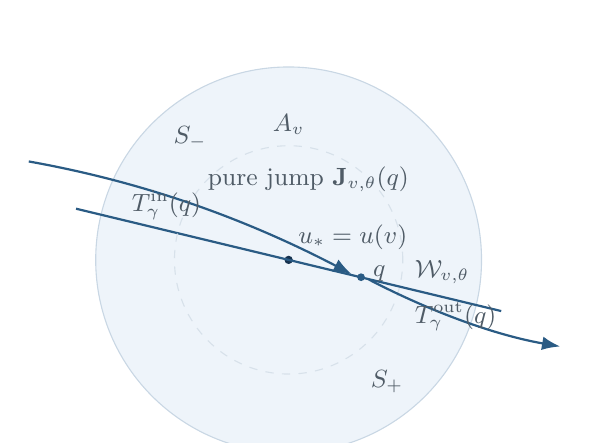
\begin{tikzpicture}[x=1cm,y=1cm,>=Latex]
  \draw[LineBlue,fill=SoftBlue] (0,0) circle (2.45);
  \fill[TitleBlue] (0,0) circle (1.5pt);
  \node[font=\small,text=MutedText,above right] at (0,0) {$u_*=u(v)$};
  \draw[AccentBlue,thick] (-2.7,0.65) -- (2.7,-0.65);
  \node[font=\small,text=MutedText] at (1.95,-0.15) {$\wall_{v,\theta}$};
  \node[font=\small,text=MutedText] at (-1.25,1.55) {$S_-$};
  \node[font=\small,text=MutedText] at (1.25,-1.55) {$S_+$};
  \draw[RuleGray,dashed] (0,0) circle (1.45);
  \node[font=\small,text=MutedText] at (0,1.72) {$A_v$};
  \fill[AccentBlue] (0.92,-0.22) circle (1.4pt);
  \node[font=\small,text=MutedText,right] at (0.95,-0.18) {$q$};
  \draw[AccentBlue,thick,-Latex] (-3.3,1.25) .. controls (-1.9,1.0) and (-0.6,0.55) .. (0.80,-0.18);
  \draw[AccentBlue,thick,-Latex] (1.02,-0.25) .. controls (1.85,-0.68) and (2.65,-0.96) .. (3.45,-1.10);
  \node[font=\small,text=MutedText] at (-1.55,0.70) {$\Tin(q)$};
  \node[font=\small,text=MutedText] at (2.12,-0.72) {$\Tout(q)$};
  \node[font=\small,text=MutedText,align=center] at (0.25,1.02) {pure jump\ $\Jemb(q)$};
\end{tikzpicture}
\caption{Local-to-global factorization at one active selector point. The path is propagated to an admissible overlap point $q$ in the entry sector, the pure selector block is inserted there, and propagation then continues in the exit sector.}
\end{figure}

\section{The exact local-to-global theorem}

\subsection{Statement}

\begin{theorem}[Exact local-to-global theorem]
\label{thm:local-to-global}
Let $s$ be the active selector point determined by a generic simple phase-active transport ramification point $v$, and let $\gamma$ be a continuation path crossing the associated selector wall once and transversely inside an admissible selector disk $D_v$.

Then the exact global insertion rule of Definition~\ref{def:global-insertion-rule} exists. More precisely:
\begin{enumerate}
  \item for every admissible overlap point $q\in A_v$, the pure local selector jump is
  \begin{equation}
  \label{eq:Jemb-main}
  \Jemb(q;H)=\iota_v\!\bigl(I+s^{\mathrm{BS}}_{v,\theta}(q;H)N_{v,\theta}\bigr);
  \end{equation}
  \item the full continuation matrix factors exactly as
  \begin{equation}
  \label{eq:factor-main}
  \Tfun_\gamma(H,\theta)=\Tout(q;H,\theta)\,\Jemb(q;H)\,\Tin(q;H,\theta);
  \end{equation}
  \item if $q,q'\in A_v$, then
  \begin{equation}
  \label{eq:J-transport-law}
  \Jemb(q';H)=D_{+,v}(q',q;H)\,\Jemb(q;H)\,D_{-,v}(q',q;H)^{-1};
  \end{equation}
  consequently the factorization \eqref{eq:factor-main} is independent of $q$, of the local overlap annulus, and of the selector-disk radius used to realize the local normalization.
\end{enumerate}
In particular, the only effect of crossing the active selector wall is the insertion of one embedded scalar local block in the active $2\oplus 1$ splitting; the spectator line is untouched by the selector jump itself.
\end{theorem}

\subsection{Preparatory lemmas}

\begin{lemma}[Local active-spectator splitting in the intrinsic frame]
\label{lem:active-spectator}
On the resolved-sheet / half-form lift of $D_v$, the exact local coefficient system splits as the direct sum of the active two-sheet system and one analytic spectator line.
\end{lemma}

\begin{proof}
The reduced sheet carriers satisfy exact scalar equations on every local sheet:
\begin{equation}
\label{eq:three-sheet-scalar}
\partial_u R_\alpha=\ii\bigl(E_\alpha-E_x\bigr)R_\alpha,
\qquad
\alpha\in\{+,-,\mathrm{sp}\}.
\end{equation}
At a simple selector point, two of these sheets collide and form the active pair; the third remains separated by hypothesis. After half-form reconstruction, each sheet still contributes one scalar local coefficient. Therefore the exact local coefficient frame is diagonal in the ordered basis $(L_+,L_-,L_{\mathrm{sp}})$, and the spectator line remains analytic through the whole selector disk. This yields the direct-sum local coefficient system
\[
(L_+\oplus L_-)\oplus L_{\mathrm{sp}}.
\]
\end{proof}

\begin{lemma}[Embedded local selector block]
\label{lem:embedded-block}
For every admissible overlap point $q\in A_v$, the coefficient jump across the selector wall is exactly the embedded active block
\begin{equation}
\label{eq:embedded-block}
\Jemb(q;H)=\iota_v\bigl(\Jact(q;H)\bigr)=\iota_v\!\bigl(I+s^{\mathrm{BS}}_{v,\theta}(q;H)N_{v,\theta}\bigr).
\end{equation}
\end{lemma}

\begin{proof}
By the intrinsic bridge lemma, after resolved-sheet lift and half-form regularization the quotient-ring / adiabatic exact local frame agrees with the canonical resolved-sheet exact frame, up to one constant geometry-only matrix and identically in matched normalization. Therefore the active local coefficient jump is precisely the one proved in the generic simple local sufficiency theorem:
\[
\Jact(q;H)=I+s^{\mathrm{BS}}_{v,\theta}(q;H)N_{v,\theta}.
\]
By Lemma~\ref{lem:active-spectator}, the spectator line is analytic across the selector wall and carries no sector jump. Using the same spectator frame on both sides of the wall, the coefficient jump on the spectator factor is the identity. Hence the full local block is the direct sum of the active jump and the identity on the spectator line, i.e. \eqref{eq:embedded-block}.
\end{proof}

\begin{lemma}[Transport law for the local selector block]
\label{lem:transport-law}
For $q,q'\in A_v$, the embedded selector blocks are related by
\begin{equation}
\label{eq:transport-law-lemma}
\Jemb(q';H)=D_{+,v}(q',q;H)\,\Jemb(q;H)\,D_{-,v}(q',q;H)^{-1}.
\end{equation}
\end{lemma}

\begin{proof}
Let $c_-(q)$ and $c_+(q)$ denote coefficient vectors in the entry- and exit-sector exact local frames at $q$. By definition of the local selector jump,
\begin{equation}
\label{eq:jump-coeff-def}
 c_+(q)=\Jemb(q;H)c_-(q).
\end{equation}
Propagating from $q$ to $q'$ inside the two sectors gives
\[
 c_-(q')=D_{-,v}(q',q;H)c_-(q),
 \qquad
 c_+(q')=D_{+,v}(q',q;H)c_+(q).
\]
Substituting \eqref{eq:jump-coeff-def} into the second identity yields
\[
 c_+(q')=D_{+,v}(q',q;H)\,\Jemb(q;H)\,D_{-,v}(q',q;H)^{-1}c_-(q').
\]
But the coefficient jump at $q'$ is by definition $c_+(q')=\Jemb(q';H)c_-(q')$. Comparing the two expressions proves \eqref{eq:transport-law-lemma}.
\end{proof}

\subsection{Proof of the theorem}

\begin{proof}[Proof of Theorem~\ref{thm:local-to-global}]
Part (1) is exactly Lemma~\ref{lem:embedded-block}.

For part (2), choose an admissible overlap point $q\in A_v$. Split the global path at the crossing into the segment before the selector wall and the segment after the selector wall, both cut at $q$. By definition, $\Tin(q;H,\theta)$ is the exact coefficient propagator along the part of $\gamma$ before the crossing, written in the entry-sector frame at $q$, and $\Tout(q;H,\theta)$ is the exact coefficient propagator along the part of $\gamma$ after the crossing, written in the exit-sector frame at $q$. The coefficient vector therefore evolves as
\[
 c_{\mathrm{final}}
 =\Tout(q;H,\theta)\,c_+(q)
 =\Tout(q;H,\theta)\,\Jemb(q;H)\,c_-(q)
 =\Tout(q;H,\theta)\,\Jemb(q;H)\,\Tin(q;H,\theta)c_{\mathrm{initial}}.
\]
Since this holds for every initial coefficient vector, we obtain the exact factorization
\[
 \Tfun_\gamma(H,\theta)=\Tout(q;H,\theta)\,\Jemb(q;H)\,\Tin(q;H,\theta).
\]

For part (3), let $q,q'\in A_v$. By multiplicativity of coefficient propagation,
\begin{equation}
\label{eq:Tin-Tout-change}
 \Tin(q';H,\theta)=D_{-,v}(q',q;H)\,\Tin(q;H,\theta),
 \qquad
 \Tout(q;H,\theta)=\Tout(q';H,\theta)\,D_{+,v}(q',q;H).
\end{equation}
Using Lemma~\ref{lem:transport-law} and \eqref{eq:Tin-Tout-change}, we compute
\begin{align*}
 \Tout(q';H,\theta)\,\Jemb(q';H)\,\Tin(q';H,\theta)
 &=\Tout(q';H,\theta)
   D_{+,v}(q',q;H)\,\Jemb(q;H)\,D_{-,v}(q',q;H)^{-1}
   D_{-,v}(q',q;H)\,\Tin(q;H,\theta)\\
 &=\Tout(q;H,\theta)\,\Jemb(q;H)\,\Tin(q;H,\theta).
\end{align*}
Therefore the factorization is independent of the overlap point. Moving the overlap point radially or changing the overlap annulus is a special case of the same transport law, so the right-hand side is independent of all local choices.

This proves the exact global insertion rule.
\end{proof}

\begin{remark}[What is and is not inside the selector block]
The selector block is the \emph{pure wall-crossing factor} at a fixed admissible overlap point. All regular local evolution before or after that point -- including any diagonal or spectator propagation inside the selector disk -- belongs to the adjacent ordinary propagators $\Tin$ and $\Tout$, not to $\Jemb$. This is why the spectator line appears with the identity inside the selector block even though the spectator coefficient certainly evolves along the surrounding path.
\end{remark}

\section{Corollaries}

\subsection{Ordered-product continuation functor}

\begin{corollary}[Ordered-product continuation word]
\label{cor:ordered-product}
Let $\gamma$ be a continuation path whose decorated word meets ordinary edges $e_0,e_1,\dots,e_m$ and active selector points $s_1,s_2,\dots,s_m$ in that order. Choose any admissible overlap point $q_k$ for each $s_k$, and let $D_{e_k}(H,\theta)$ denote the exact ordinary coefficient propagator on the $k$th edge segment. Then
\begin{equation}
\label{eq:ordered-product}
\Tfun_\gamma(H,\theta)=D_{e_m}(H,\theta)\,\mathbf J_{s_m}(q_m;H)\,D_{e_{m-1}}(H,\theta)\cdots
\mathbf J_{s_1}(q_1;H)\,D_{e_0}(H,\theta).
\end{equation}
The product is independent of the overlap choices $q_k$.
\end{corollary}

\begin{proof}
Apply Theorem~\ref{thm:local-to-global} successively at each selector crossing and use path multiplicativity \eqref{eq:path-mult}. Independence of the $q_k$ follows pointwise from part (3) of the theorem.
\end{proof}

\subsection{Explicit resolution of the broken morphism $j_{H,\theta}$}

The strategy diagram isolated a broken morphism
\[
 j_{H,\theta}:\Selcand\dashrightarrow J_{H,\theta}
\]
that was supposed to turn candidate selector points into actual active points equipped with local jump matrices. In the generic simple regime, the theorem above makes this explicit.

\begin{corollary}[Explicit local activation--multiplier morphism]
\label{cor:j-explicit}
For a simple phase-active candidate selector point $s$ attached to $v$, define the vertex label
\begin{equation}
\label{eq:Jclass-def}
\Jclass:=\bigl[ q\longmapsto \Jemb(q;H)\bigr],
\end{equation}
where the brackets denote the transport equivalence of Theorem~\ref{thm:local-to-global}(3). Then the broken morphism is resolved by
\begin{equation}
\label{eq:j-explicit}
 j_{H,\theta}(s)=\Jclass.
\end{equation}
Equivalently, the local activation--multiplier object is now explicit in the generic simple case.
\end{corollary}

\begin{proof}
Local selector sufficiency identifies the actual active subset with the phase-active simple ramification points. Theorem~\ref{thm:local-to-global} assigns to each such point the well-defined transport-equivalence class of embedded scalar local blocks. This is exactly the data that $j_{H,\theta}$ was meant to provide.
\end{proof}

\subsection{Translation to other exact local frames}

\begin{corollary}[Constant-conjugacy transport to any exact local frame]
\label{cor:constant-conjugacy}
Let $Y^{\mathrm{other}}_v$ be any other exact local frame that differs from the intrinsic resolved-sheet / half-form frame by one constant geometry-only matrix $G_v$. Then the selector block in that frame is
\begin{equation}
\label{eq:other-frame}
\Jemb^{\mathrm{other}}(q;H)=\widetilde G_v^{-1}\,\Jemb(q;H)\,\widetilde G_v,
\qquad
\widetilde G_v:=G_v\oplus 1.
\end{equation}
With the matched normalization of the bridge lemma one has $G_v=I$, hence $\Jemb^{\mathrm{other}}=\Jemb$.
\end{corollary}

\begin{proof}
This is immediate from the intrinsic bridge theorem: changing exact local frame by a constant matrix conjugates every coefficient jump by the same constant matrix. The spectator factor remains untouched, so the conjugating matrix is $\widetilde G_v=G_v\oplus 1$.
\end{proof}

\begin{figure}[H]
\centering
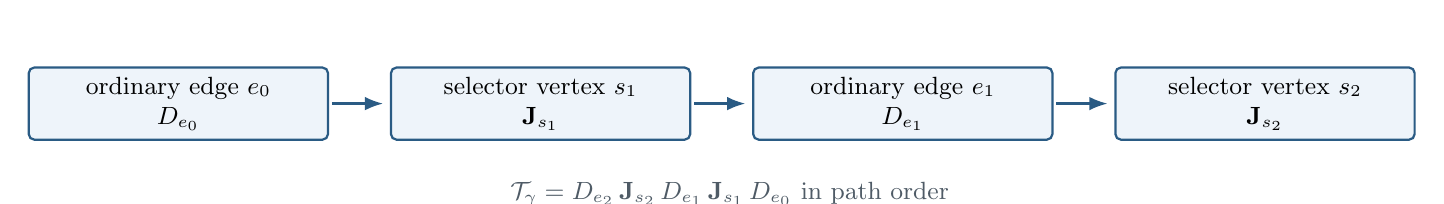
\begin{tikzpicture}[x=1cm,y=1cm,>=Latex]
  \node[draw=AccentBlue,rounded corners=2pt,thick,fill=SoftBlue,minimum width=3.8cm,minimum height=0.9cm,align=center,font=\small] (e0) at (0,0) {ordinary edge $e_0$\\$D_{e_0}$};
  \node[draw=AccentBlue,rounded corners=2pt,thick,fill=SoftBlue,minimum width=3.8cm,minimum height=0.9cm,align=center,font=\small] (s1) at (4.6,0) {selector vertex $s_1$\\$\mathbf J_{s_1}$};
  \node[draw=AccentBlue,rounded corners=2pt,thick,fill=SoftBlue,minimum width=3.8cm,minimum height=0.9cm,align=center,font=\small] (e1) at (9.2,0) {ordinary edge $e_1$\\$D_{e_1}$};
  \node[draw=AccentBlue,rounded corners=2pt,thick,fill=SoftBlue,minimum width=3.8cm,minimum height=0.9cm,align=center,font=\small] (s2) at (13.8,0) {selector vertex $s_2$\\$\mathbf J_{s_2}$};
  \draw[AccentBlue,thick,-Latex] (1.95,0) -- (2.6,0);
  \draw[AccentBlue,thick,-Latex] (6.55,0) -- (7.2,0);
  \draw[AccentBlue,thick,-Latex] (11.15,0) -- (11.8,0);
  \node[font=\small,text=MutedText] at (7.0,-1.15) {$\Tfun_\gamma = D_{e_2}\,\mathbf J_{s_2}\,D_{e_1}\,\mathbf J_{s_1}\,D_{e_0}$ in path order};
\end{tikzpicture}
\caption{Once the local selector block is known, the continuation functor becomes the ordered product of ordinary edge propagators and embedded selector blocks.}
\end{figure}

\section{Theorem-shaping numerical assays}

The proof above is symbolic. The numerical assays were useful only in sharpening the generic hypotheses and in building confidence that the theorem should be true before the symbolic closure was found.

\begin{longtable}{P{0.27\textwidth}P{0.13\textwidth}P{0.15\textwidth}P{0.31\textwidth}} 
\caption{Numerical assays that were most useful in shaping the theorem statement.}\\
\toprule
\textbf{Assay} & \textbf{Precision} & \textbf{Accepted samples} & \textbf{Use in theorem shaping} \\
\midrule
\endfirsthead
\toprule
\textbf{Assay} & \textbf{Precision} & \textbf{Accepted samples} & \textbf{Use in theorem shaping} \\
\midrule
\endhead
Resolved-sheet off-diagonal probe & 80 digits & 1200 & No off-diagonal counterexample found. Helped isolate the intrinsic torus statement as the correct local normal form. \\
Spectator-decoupled torus survival & 80 digits & 1001 (including 301 targeted high-curvature) & 1001/1001 pass. Supported the belief that no hidden local selector mixing with the spectator survives in the intrinsic normalization. \\
Sector-independence of residual constant part & 80 digits base, 100 digits refined retest & 1001 & 999/1001 base passes; both borderline misses pass 100-digit retest. Helped justify treating the bridge as constant-conjugacy data rather than a fresh local matrix problem. \\
Selector sufficiency random assay & 60 digits & 1302 & 1302/1302 accepted-sample passes, no counterexample. Strongly suggested that every simple phase-active point really does carry the local scalar block. \\
Selector sufficiency replay / audit & 70 digits & 1302 replayed & 1302/1302 recomputed passes, no replay failures. Confirmed that the local activation premise was not a transient numerical artifact. \\
\bottomrule
\end{longtable}

The numerical artifacts most directly tied to the selector sufficiency assay and its replay were generated earlier in the conversation and include the logged workbook, accepted-sample CSV, replay script, replay summary JSON, replay report, and combined replay log.

\section{Status after the theorem}

Excluding nongeneric collision scenarios, the symbolic agenda is now closed.

\begin{itemize}
  \item The common cover, spinor lift, quotient-ring reduction, commuting triple, and canonical gluing are formalized.
  \item The canonical exact two-sheet gauge is torus-valued to all orders.
  \item The intrinsic bridge to the quotient-ring / adiabatic half-form frame is constant and geometry-only.
  \item Simple phase-active transport ramification points are genuine local selector points.
  \item The exact local-to-global theorem proved here places the scalar local block into the continuation functor by an explicit embedded insertion rule.
\end{itemize}

So, in the generic simple regime, the only remaining work is nongeneric: degenerate transport ramification, common $Q_4$-$W_4$ collisions, collisions with ordinary turning points, and other topology-changing limits.

\section{Conclusion}

The exact global insertion rule can be summarized in one sentence:
\begin{quote}\itshape
for a simple phase-active selector point, the global continuation matrix is obtained by inserting exactly one embedded scalar local block in the active $2\oplus 1$ splitting, with the spectator line untouched by the selector jump itself, and the resulting product is independent of all local overlap choices.
\end{quote}

This is precisely the local-to-global statement that had remained open in the formal strategy diagram. In the generic simple regime, the broken morphism $j_{H,\theta}$ is now explicit, and the continuation functor is fully determined by ordinary edge propagation together with the embedded scalar selector vertices.

\begin{thebibliography}{99}

\bibitem{LZSummary}
\emph{Multistate Landau-Zener Solver: Augmented ODE with Gauged Dynamics} (internal summary).

\bibitem{GapNote}
\emph{A note on the sextic gap polynomial for $N=3$ Type-1 matrices} (internal note).

\bibitem{Primer}
\emph{Type-1, $N=3$ Landau-Zener primer: double cover, reduced ODE, gluing theorem, and selector} (internal primer).

\bibitem{Strategy}
\emph{Formalized strategy diagram for Type-1, $N=3$ Landau-Zener} (internal note).

\bibitem{LocalMatching}
\emph{Local selector matching at a transport ramification point in Type-1, $N=3$} (internal note, April 16, 2026).

\bibitem{TransportPhase}
\emph{Transport versus phase in the local gauge expansion at a simple transport ramification point} (internal note, April 17, 2026).

\bibitem{MainApril18}
\emph{All-orders torus structure and affine-linear local phase recurrences in Type-1, $N=3$ Landau-Zener} (main text draft, April 18, 2026).

\bibitem{SuppApril18}
\emph{Technical Supplement: all-orders torus structure, phase recurrence, and numerical support} (supplement draft, April 18, 2026).

\bibitem{Memorial}
\emph{Selector sufficiency and outer-frame descent in Type-1, $N=3$ Landau-Zener} (conversation memorial note, April 19, 2026).

\bibitem{SelectorAssay}
Selector sufficiency assay artifacts generated in the conversation: the logged workbook, accepted-sample CSV, summary JSON, plain-text report, and companion CSV files.

\bibitem{SelectorReplay}
Selector sufficiency replay artifacts generated in the conversation: the replay script, replay report, replay summary JSON, combined replay log, and companion replay CSV files.

\end{thebibliography}

\end{document}
